\documentclass[compress]{beamer}
\usepackage{ifthen,verbatim}

\newcommand{\isnote}{}
\xdefinecolor{lightyellow}{rgb}{1.,1.,0.25}
\xdefinecolor{darkblue}{rgb}{0.1,0.1,0.7}

%% Uncomment this to get annotations
%% \def\notes{\addtocounter{page}{-1}
%%            \renewcommand{\isnote}{*}
%% 	   \beamertemplateshadingbackground{lightyellow}{white}
%%            \begin{frame}
%%            \frametitle{Notes for the previous page (page \insertpagenumber)}
%%            \itemize}
%% \def\endnotes{\enditemize
%% 	      \end{frame}
%%               \beamertemplateshadingbackground{white}{white}
%%               \renewcommand{\isnote}{}}

%% Uncomment this to not get annotations
\def\notes{\comment}
\def\endnotes{\endcomment}

\setbeamertemplate{navigation symbols}{}
\setbeamertemplate{headline}{\mbox{ } \hfill
\begin{minipage}{5.5 cm}
\vspace{-0.75 cm} \small
\end{minipage} \hfill
\begin{minipage}{4.5 cm}
\vspace{-0.75 cm} \small
\begin{flushright}
\ifthenelse{\equal{\insertpagenumber}{1}}{}{Jim Pivarski \hspace{0.2 cm} \insertpagenumber\isnote/\pageref{numpages}}
\end{flushright}
\end{minipage}\mbox{\hspace{0.2 cm}}\includegraphics[height=1 cm]{../cmslogo} \hspace{0.1 cm} \includegraphics[height=1 cm]{../tamulogo} \hspace{0.01 cm} \vspace{-1.05 cm}}

\begin{document}
\begin{frame}
\begin{center}
\vfill \textcolor{darkblue}{\LARGE iCSA08 Muon Alignment}

\vspace{0.5 cm} \small 7 May, 2008

\vfill \renewcommand{\arraystretch}{1.5} \begin{tabular}{c c c}
\textcolor{darkblue}{} & & \textcolor{darkblue}{Pablo Martinez} \\
\textcolor{darkblue}{Jim Pivarski} & & \textcolor{darkblue}{Francisco Matorras} \\
\textcolor{darkblue}{Alexei Safonov} & & \textcolor{darkblue}{Javier Fern\'andez} \\
\textcolor{darkblue}{} & & \textcolor{darkblue}{Rebeca Gonz\'alez} \\
\small Texas A\&M University & & \small Instituto de F\'isica de Cantabria
\end{tabular}

\end{center}
\end{frame}

%% \begin{notes}
%% \item This is the annotated version of my talk.
%% \item If you want the version that I am presenting, download the one
%% labeled ``slides'' on Indico (or just ignore these yellow pages).
%% \item The annotated version is provided for extra detail and a written
%% record of comments that I intend to make orally.
%% \item Yellow notes refer to the content on the {\it previous} page.
%% \item All other slides are identical for the two versions.
%% \end{notes}

%% \begin{frame}
%% \frametitle{Outline}
%% \begin{itemize}\setlength{\itemsep}{0.75 cm}
%% \item 
%% \end{itemize}
%% %% \hspace{-0.83 cm} \textcolor{darkblue}{\Large Outline2}
%% \end{frame}

\section*{DT Standalone Algorithm}

\begin{frame}
\mbox{\hspace{-1 cm}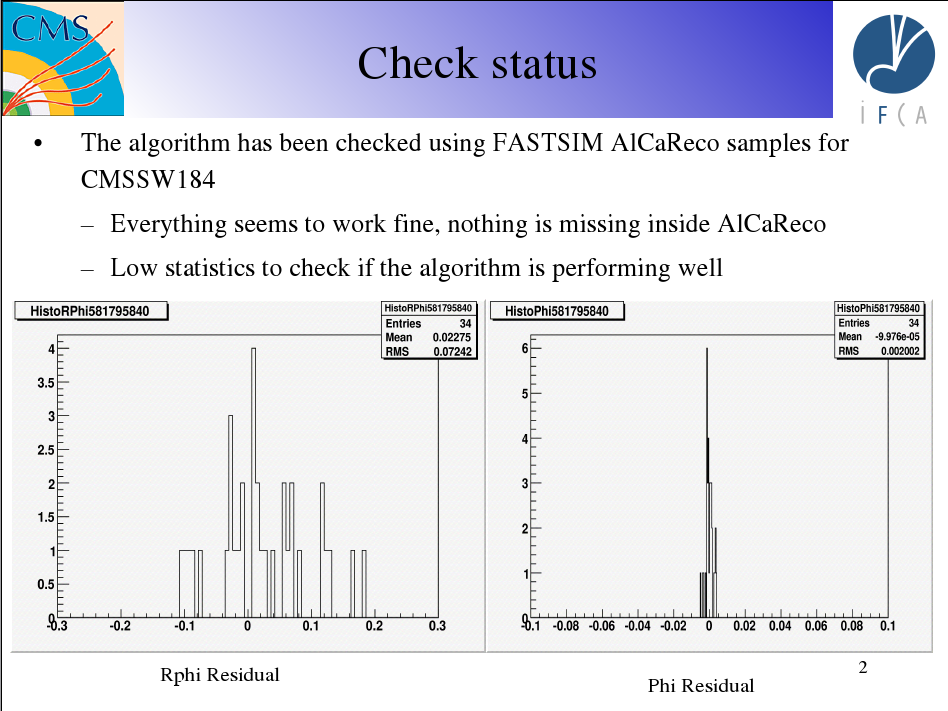
\includegraphics[width=1.2\linewidth]{pablo1.png}}
\end{frame}

\begin{frame}
\mbox{\hspace{-1 cm}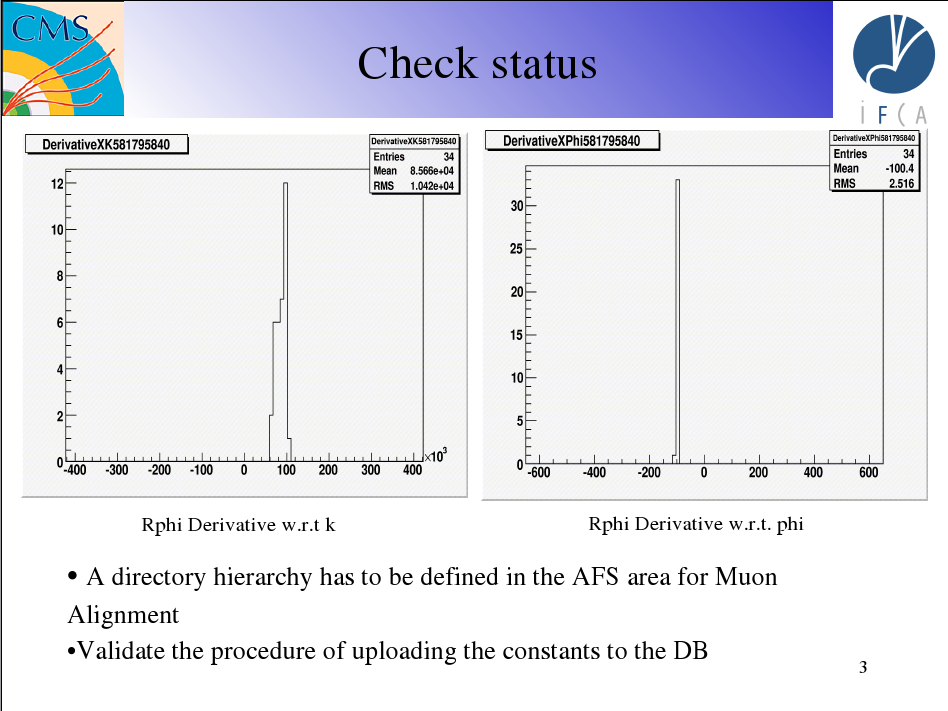
\includegraphics[width=1.2\linewidth]{pablo2.png}}
\end{frame}

\begin{frame}
\mbox{\hspace{-1 cm}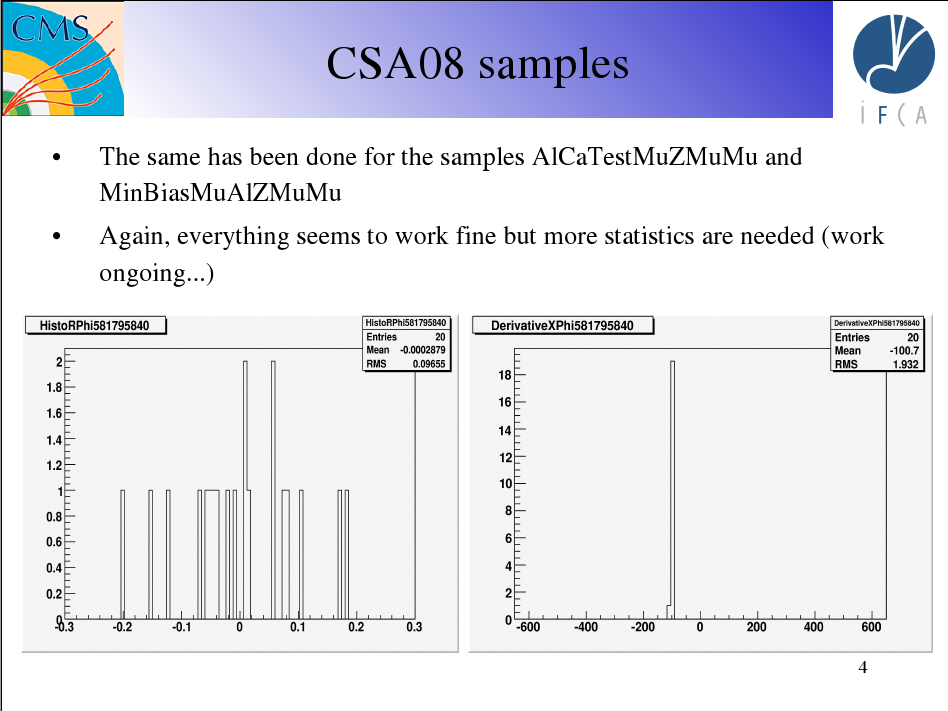
\includegraphics[width=1.2\linewidth]{pablo3.png}}
\end{frame}

\begin{frame}
\mbox{\hspace{-1 cm}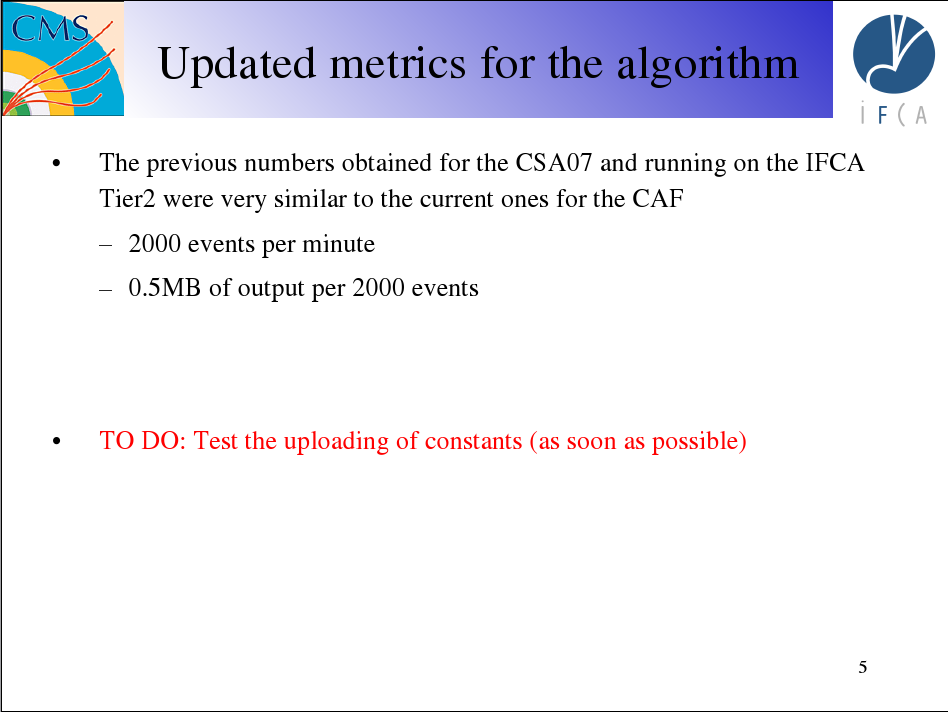
\includegraphics[width=1.2\linewidth]{pablo4.png}}
\end{frame}

\section*{Baseline HIP Algorithm}
\begin{frame}
\begin{center}
\Huge \textcolor{blue}{Baseline HIP Algorithm}
\end{center}

\vfill
\begin{itemize}
\item Cleaned up scripts and installed in ALCA\_MUONALIGN
\item Tested alignment algorithm and validation plotting in 1\_8\_4
\item Wmunu\_10TeV (46,237 events $\approx$ 7~pb$^{-1}$)
\item Layers are perfectly aligned inside chambers
\end{itemize}

\end{frame}

\begin{frame}
\frametitle{Barrel \only<1>{aligned positions}\only<2>{track residuals}}

\only<1>{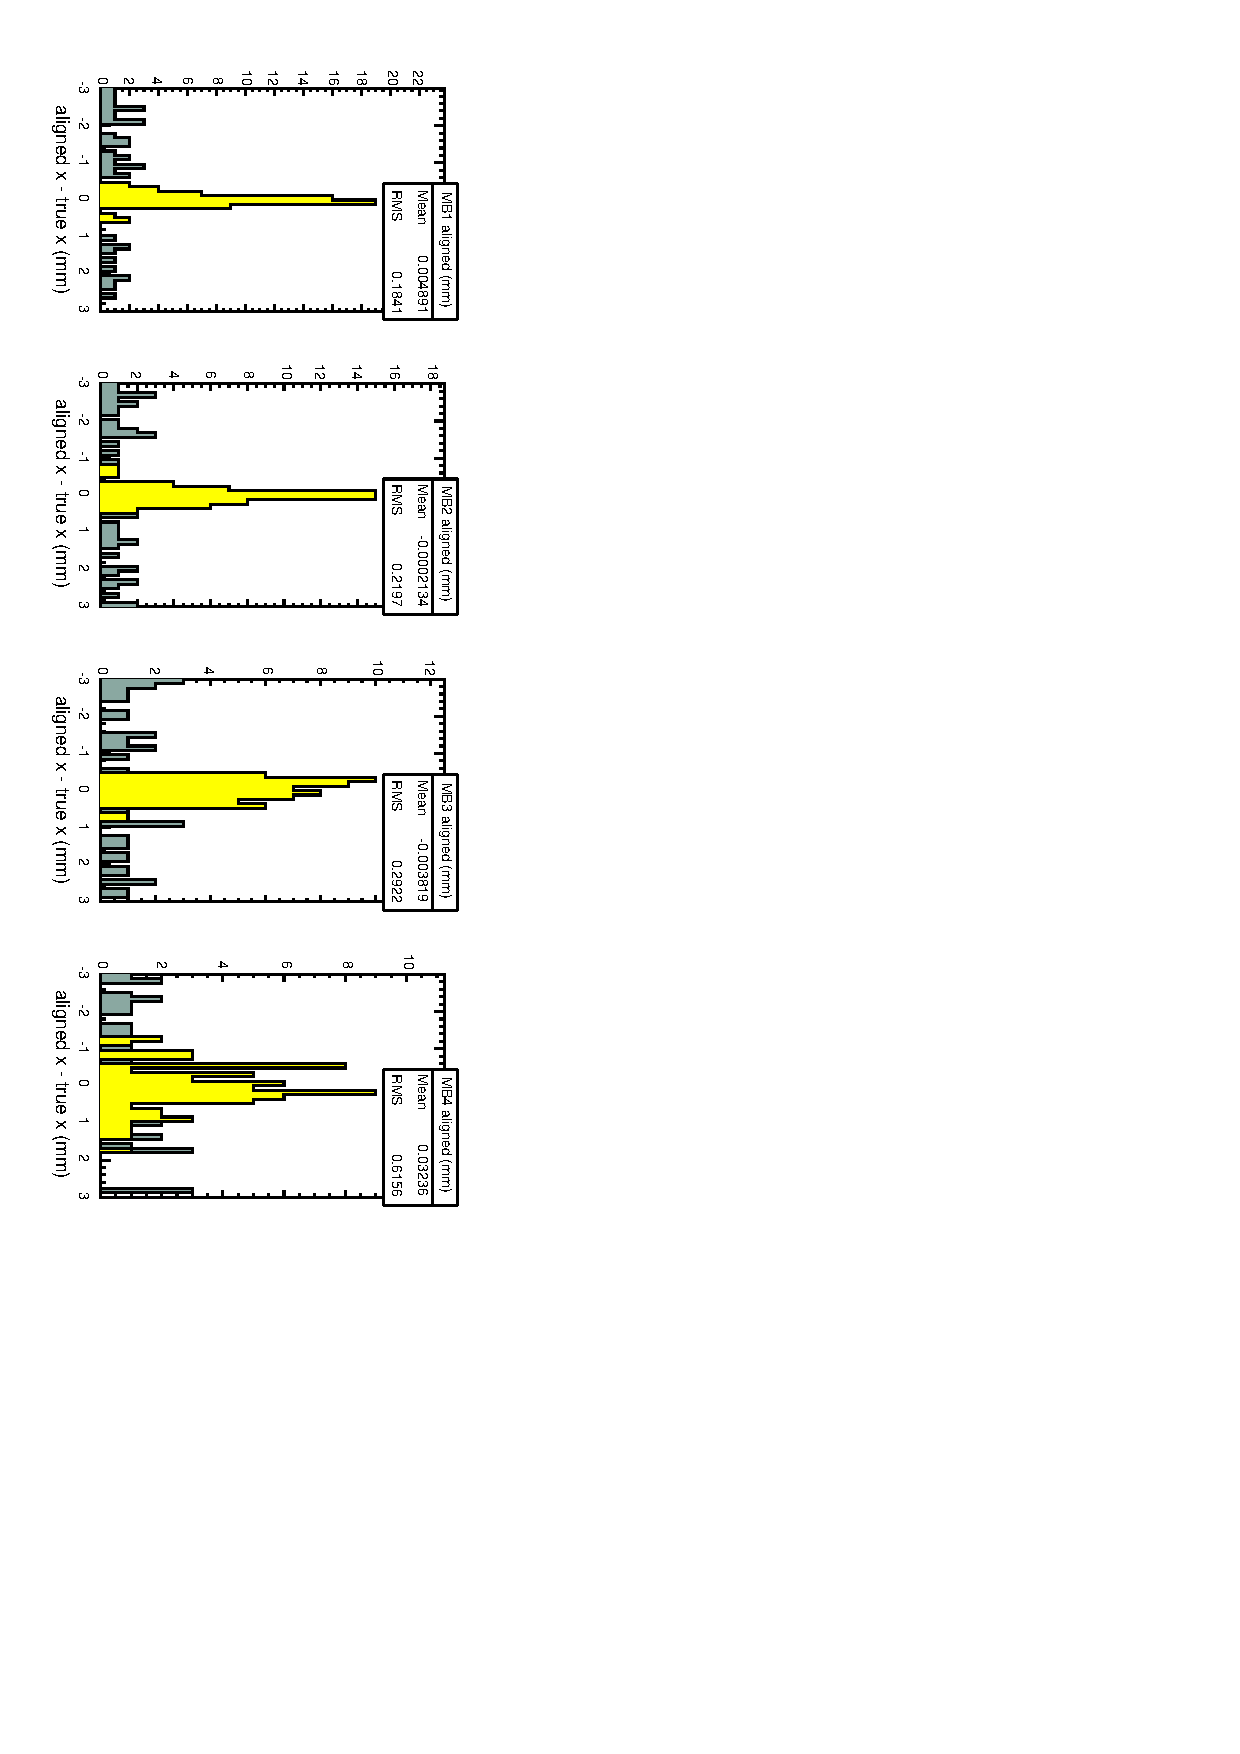
\includegraphics[height=\linewidth, angle=90]{barrel_184.pdf}}
\only<2>{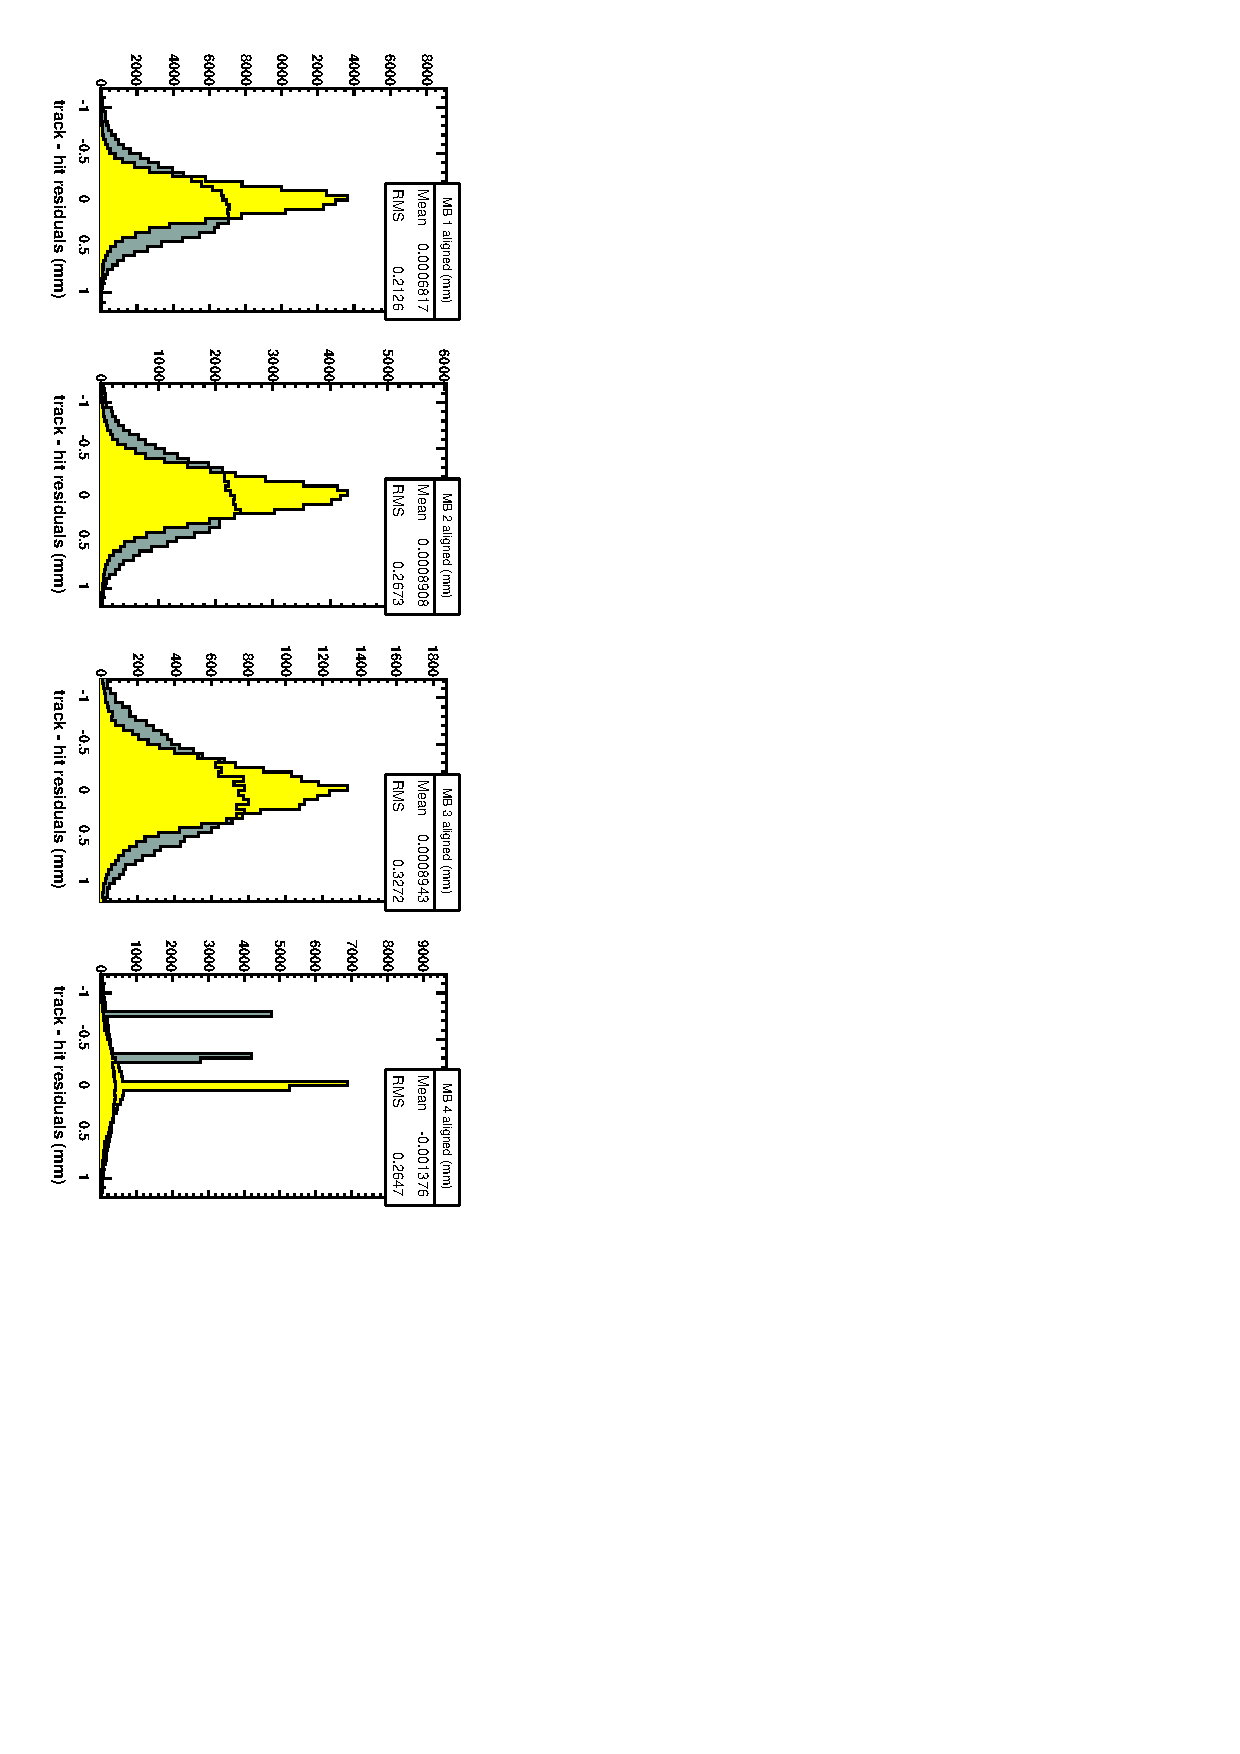
\includegraphics[height=\linewidth, angle=90]{barrel_resid_184.pdf}}

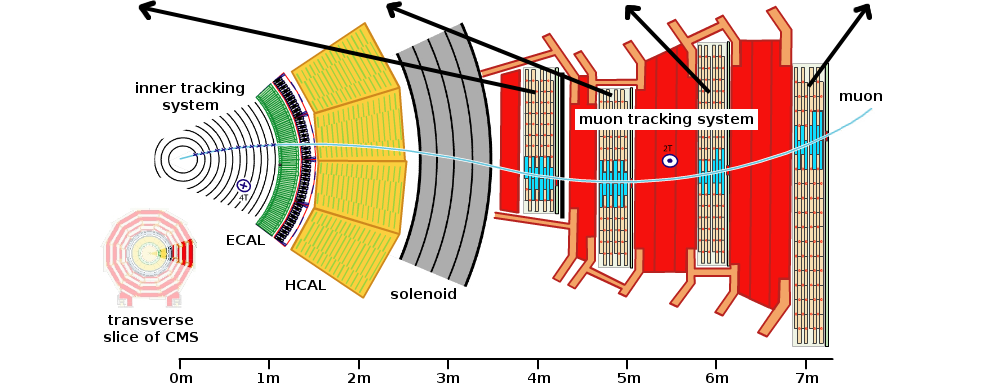
\includegraphics[width=\linewidth]{cms_slice.png}
\end{frame}

\begin{frame}
\frametitle{Endcap \only<1>{aligned positions}\only<2>{track residuals}}

\begin{columns}
\column{0.35\linewidth}
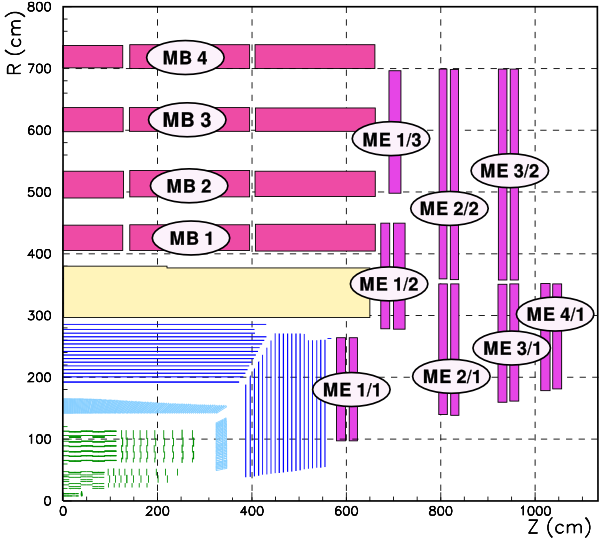
\includegraphics[width=\linewidth]{muon_system.png}
\column{0.8\linewidth}
\only<1>{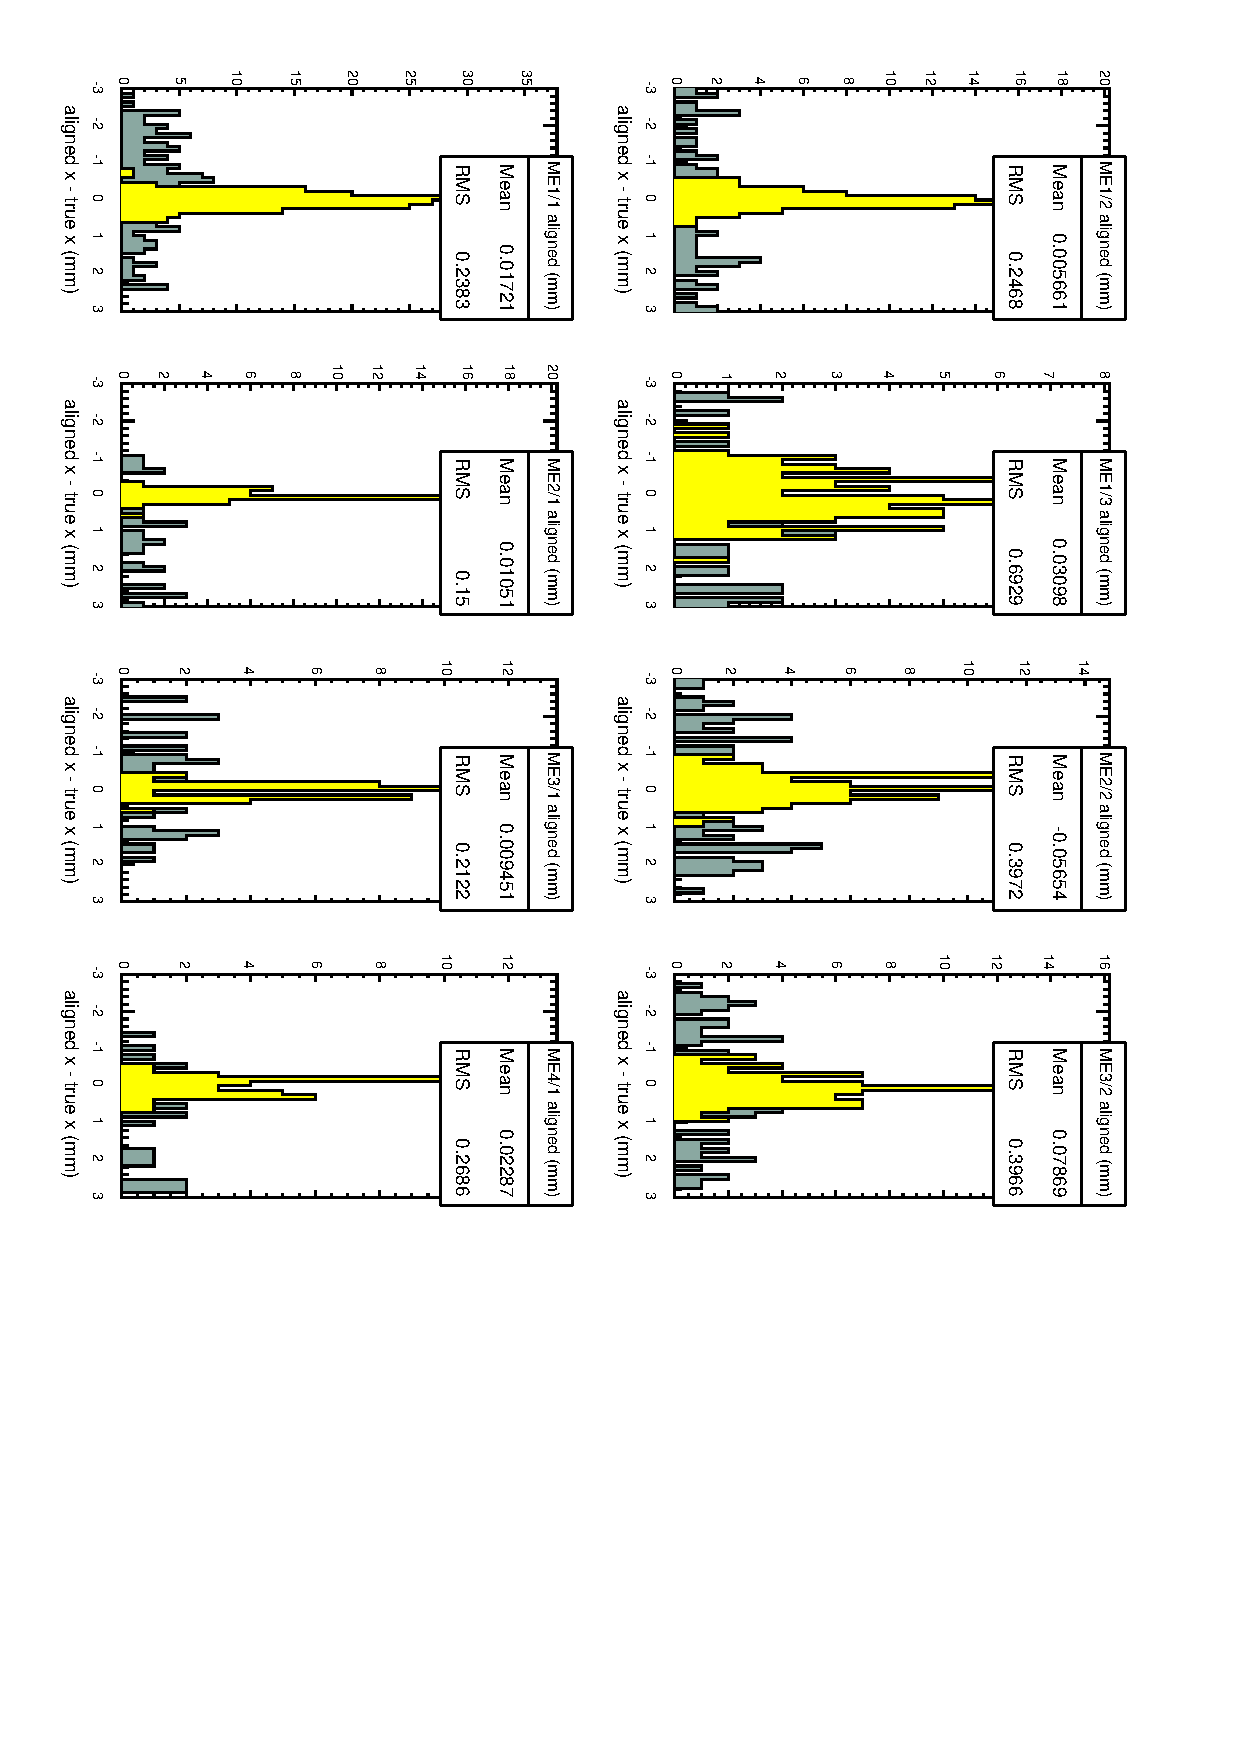
\includegraphics[height=\linewidth, angle=90]{endcap_184.pdf}}
\only<2>{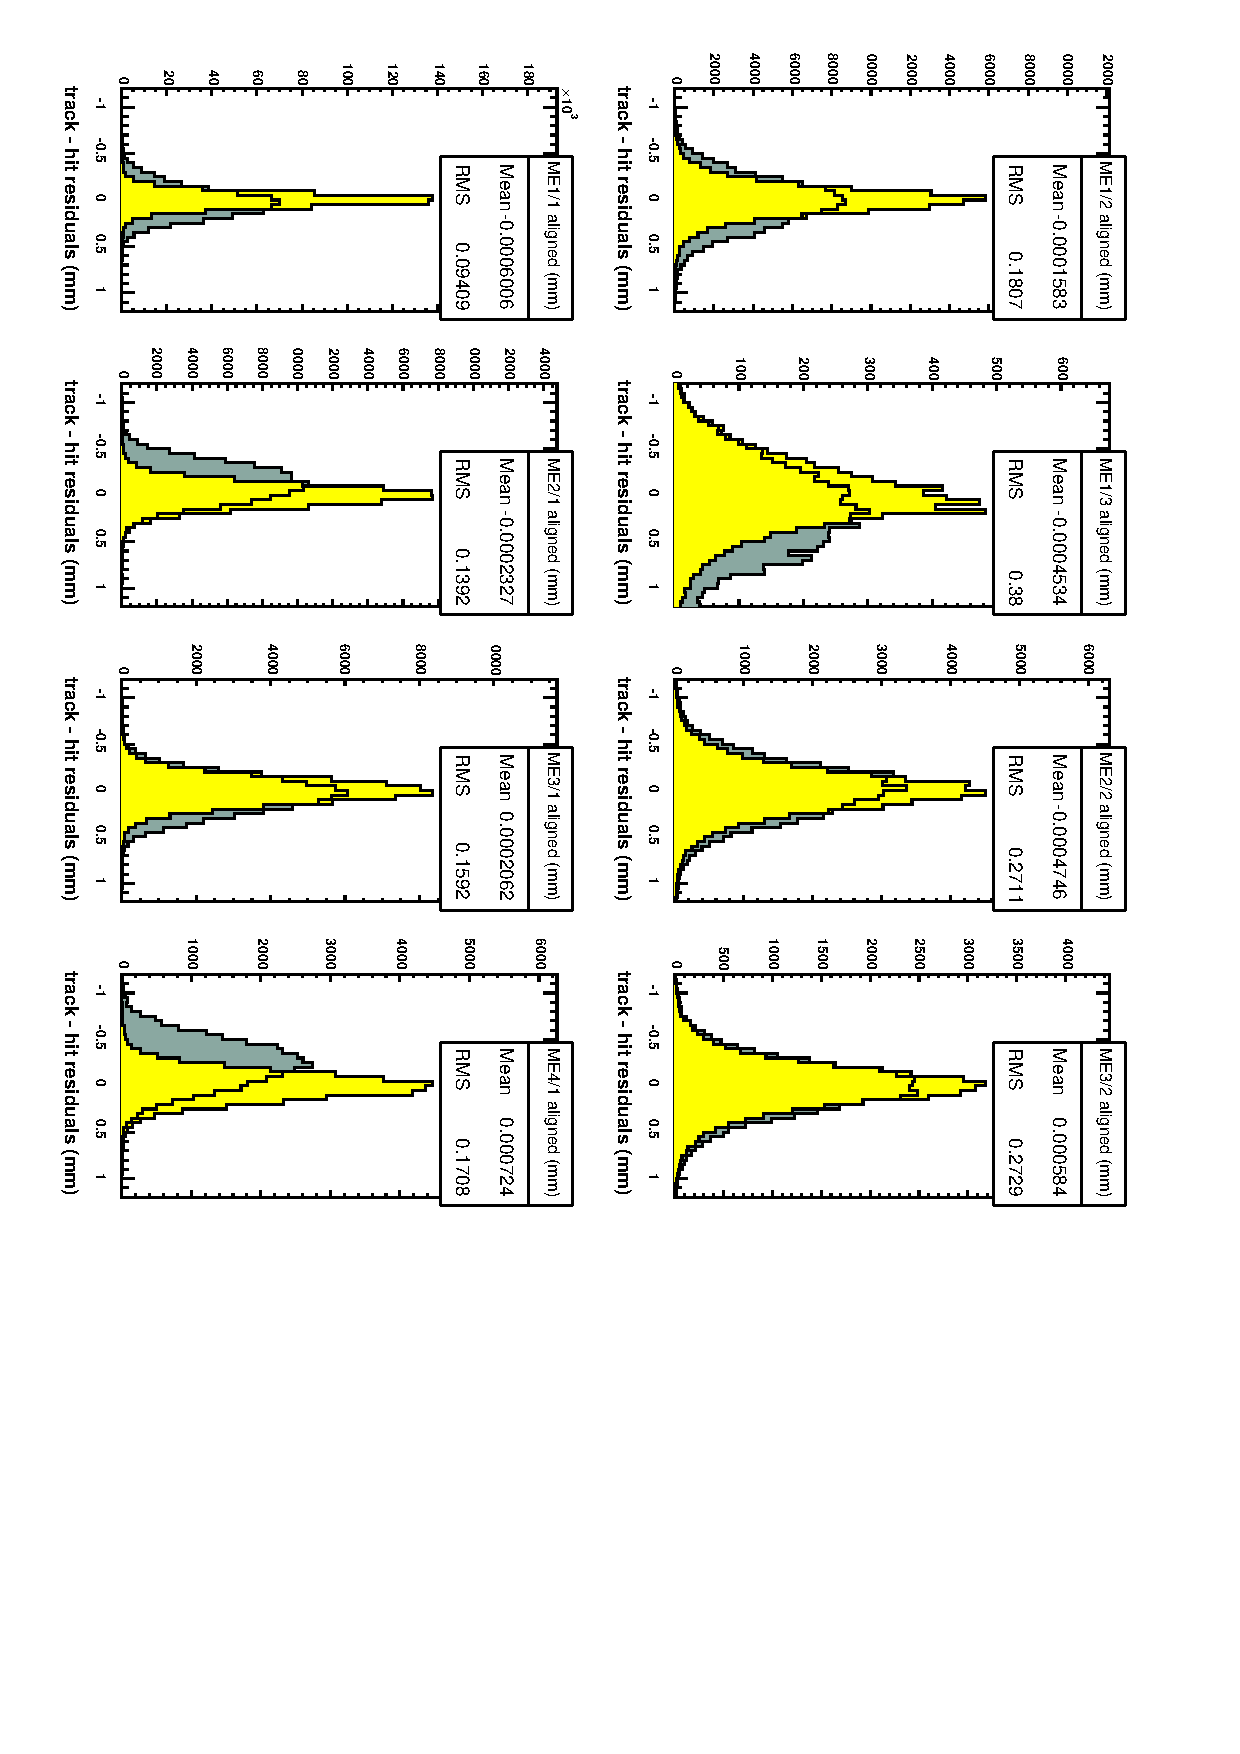
\includegraphics[height=\linewidth, angle=90]{endcap_resid_184.pdf}}
\end{columns}

\end{frame}

\begin{frame}
\frametitle{Alignment test in 2\_0\_6}

\begin{itemize}\setlength{\itemsep}{0.1 cm}
\item Minbias $\to$ muon AlCaReco was accidentally generated
\item Only 39 events; most of our low-momentum muons will come from QCD, not minbias
\item A good chance to test the 2\_0\_6 scripts
\begin{itemize}\setlength{\itemsep}{0.1 cm}
\item Fixed a bug (not loading misalignment at start of job)
\item Residuals are far too wide for our purposes
\item AlignmentProducer looped over the events, but 50 hits/chamber
are required to test alignment
\end{itemize}
\end{itemize}

\begin{center}
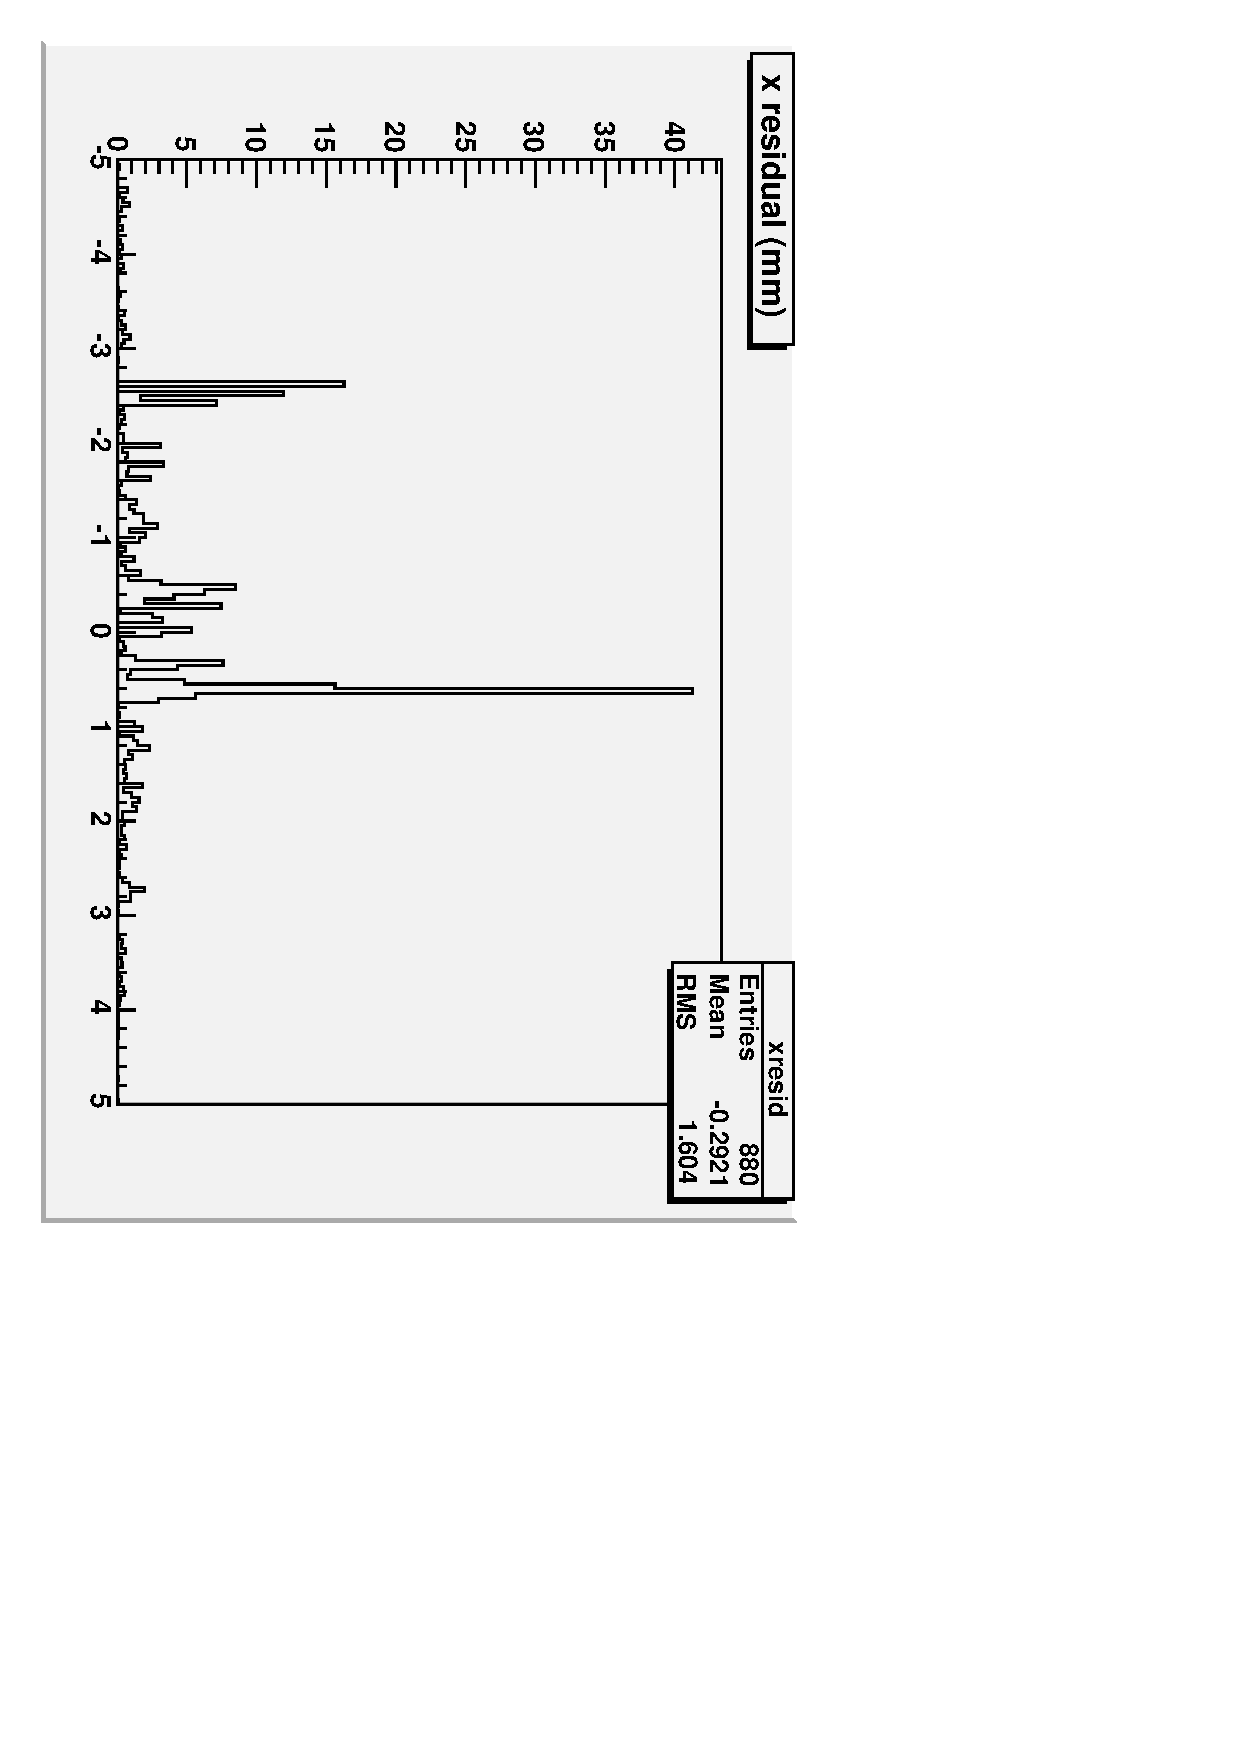
\includegraphics[height=0.6\linewidth, angle=90]{minbias_residuals.pdf}
\end{center}

\end{frame}


%% \section*{First section}
%% \begin{frame}
%% \begin{center}
%% \Huge \textcolor{blue}{First section}
%% \end{center}
%% \end{frame}

\begin{frame}
\frametitle{Conclusions}

\begin{itemize}\setlength{\itemsep}{0.4 cm}
\item Baseline procedure is the minimal goal for iCSA08
\begin{itemize}\setlength{\itemsep}{0.2 cm}
\item It is now much faster (10 hours on 50 CPUs $\to$ 4 hours on 1
CPU) because a much simpler one-pass technique yields better results
than the staged 55-pass technique
\item Not a new finding: I've been studying this for about a month,
making sure the simulation is not overoptimistic
\end{itemize}

\item Overlaps procedure (relative alignment of CSCs in rings), with
and without beam-halo is in progress
\begin{itemize}\setlength{\itemsep}{0.2 cm}
\item I have 80\% of a work-around for the AlCaReco sample containing the wrong track collections
\item Hopefully we'll have something to show for this workflow, but
our metric for success is the ``baseline'' procedure
\end{itemize}
\end{itemize}

\label{numpages}
\end{frame}

\end{document}
